\documentclass{article}
\title{Exam}
\date{31.07.2013}
\usepackage[english]{babel}
\usepackage[utf8]{inputenc}
\usepackage{enumerate}
\usepackage[cm,empty]{fullpage}
\usepackage[pdftex]{graphicx,color}
\usepackage{Sweave}
\begin{document}
\maketitle{}
\framebox{Name:\hspace{3cm}ID number:\hspace{3cm}Number of points:\hspace{2cm}STAT821 }\begin{itemize}
\item[1] {\small $\left[15\right]$ }
What is the probability of obtaining exactly 5 tails if we toss a fair coin 8 times?
\item[2] {\small $\left[15\right]$ }Data for variable nn are represented graphically.\\ 
\begin{tabular}{c}
\resizebox{50mm}{!}{
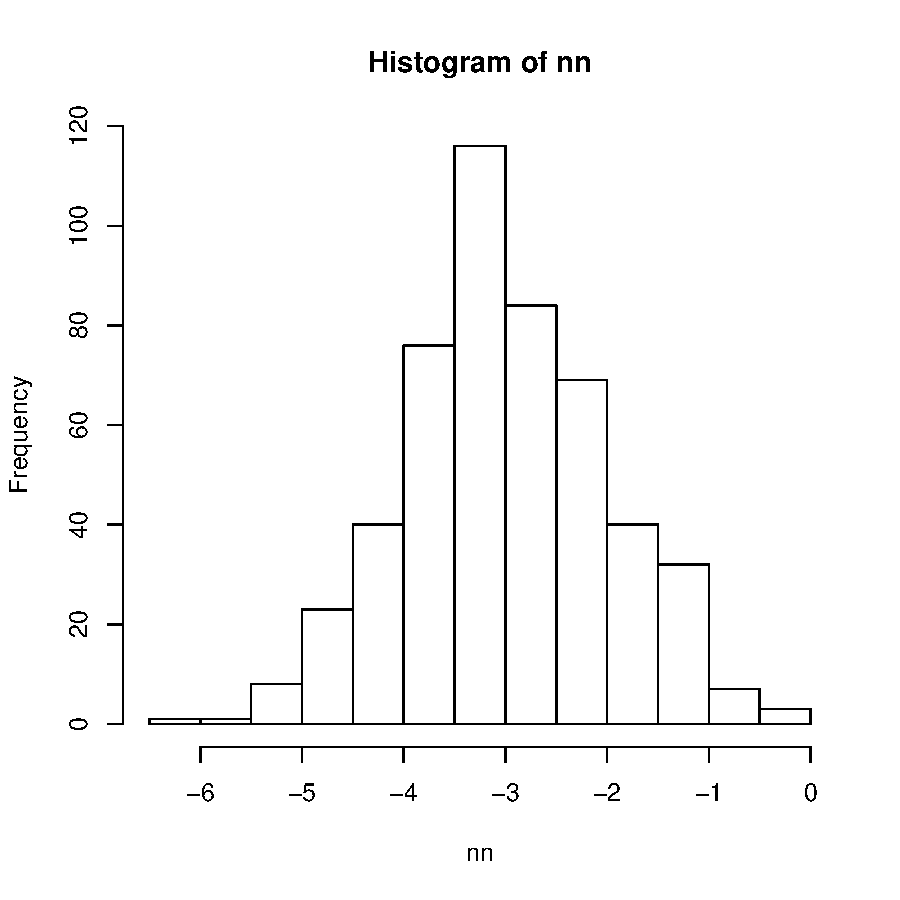
\includegraphics{exam1-002}
}
\end{tabular}

\begin{enumerate}[(a)]
\item Is standard deviation 1, 2 or 4? 
\vspace{\baselineskip}\item Is mean -3, 0 or 3? 
\vspace{\baselineskip}\end{enumerate}
\item[3] {\small $\left[15\right]$ }A genetically modified mouse does not survive the first month of life with probability 0.40.  
\begin{enumerate}[(a)]
\item We planned an experiment that included 10 mice. What is the probability that after a month not more than a mouse will survive? 
\vspace{\baselineskip} \vspace{\baselineskip} \vspace{\baselineskip}\item What is the expected number of mice still alive after the first month? 
\vspace{\baselineskip} \vspace{\baselineskip}\end{enumerate}
\item[4] {\small $\left[5\right]$ }The median value of the following data 33, 3, 7, 15, 107, 1, 41 is
\begin{enumerate}[(a)]
\item 15 
\item cannot be calculated 
\item 29.6 
\item 16 
\end{enumerate}
\end{itemize}
{\bf Good luck! }\newpage
\end{document}
